\documentclass[hyperref={bookmarks=false},aspectratio=169]{beamer}
\usepackage[utf8]{inputenc}
\usepackage{standalone}
% ---------------  Define theme and color scheme  -----------------
\usetheme[sidebarleft]{CEIT}  % 3 options: minimal, sidebarleft, sidebarright

%\setbeamertemplate{footline}[frame number]
\setbeamertemplate{footline}[text line]{%
	\parbox{\linewidth}{\vspace*{-8pt} \textcopyright \  Centre for Development of Advanced Computing (C-DAC)  \hfill \insertpagenumber}}
\setbeamertemplate{navigation symbols}{}
% ------------  Information on the title page  --------------------
\title[PPT Title]
{\bfseries{PPT Title}}

\subtitle{A brief overview}

\author[TrainerName] %\& Managed]
{TrainerName\inst{1} } %\and Managed\inst{2}}

\institute[CEIT]
{
  \inst{1}
  Trainer\\
  Centre of Excellence in IT,PNG
 % \and
 % \inst{2}
 % Trainer\\
 % Centre of Excellence in IT,PNG
}

\date[CEIT, 2014]
{Centre of Excellence in IT,PNG October 2019}
%------------------------------------------------------------

%------------------------------------------------------------
%The next block of commands puts the table of contents at the 
%beginning of each section and highlights the current section:

\AtBeginSection[]
{
  \begin{frame}
    \frametitle{Table of Contents}
    \tableofcontents[currentsection]
  \end{frame}
}

%------------------------------------------------------------


\begin{document}

\frame{\titlepage}  % Creates title page

%---------   table of contents after title page  ------------
\begin{frame}
\frametitle{Table of Contents}
\tableofcontents
\end{frame}
%---------------------------------------------------------

\section{first topic}

%---------------------------------------------------------
%Changing visivility of the text
\begin{frame}
\frametitle{frame title 1}
Every Halloween, Dabney House conducts the infamous ``Millikan pumpkin-drop experiment'' from the top of Millikan Library, the highest point on campus.

\begin{itemize}
    \item<1-> A claim was once made that the shattering of a pumpkin frozen in liquid nitrogen and dropped from a sufficient height would produce a triboluminescent spark. 
    \item<2-> This yearly event involves a crowd of observers, who try to spot the elusive spark.
    \item<3-> The title of the event is an oblique reference to the famous Millikan oil-drop experiment which measured $e$, the elemental unit of electrical charge.
\end{itemize}

\end{frame}

\begin{frame}
\frametitle{Frame Title 2}
\begin{figure}
    \centering
    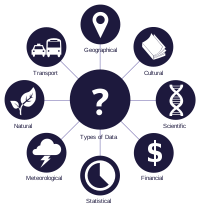
\includegraphics[width=400pt,height=210pt]{figures/fig1.png}
    \caption{``Hollywood is still mad about that, author of \emph{Legends of tech III: Techer In the Dark.}}
    \label{fig:hollywood}
\end{figure}

\end{frame}
%---------------------------------------------------------
\section{Internet of Things}
\begin{frame}
	\frametitle{Certificate Course in Internet of Things}
	\begin{columns}
		
	\column{0.45\textwidth}
			
		\begin{figure}
			
\includegraphics[width=200pt,height=150pt]{figures/course_iot.jpg}
		\end{figure}
	
	\column{0.55\textwidth}

	\begin{block}{Description}
	
		\begin{enumerate}
			\item Embedded	Linux to develop for IoT. 
			\item Wireless Network \& Communication protocols.
			\item IoT prototyping using NodeJS and Python for development.
			\item Cloud Platforms for IoT.
		\end{enumerate}
	  	  
	\end{block}

	\end{columns}
\end{frame}








%---------------------------------------------------------

%Two columns
\begin{frame}
\frametitle{Frame Title 4}

\begin{columns}

\column{0.45\textwidth}

\begin{figure}
    \centering
    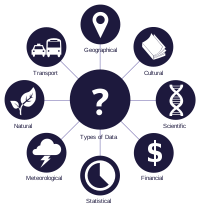
\includegraphics[scale=.4]{figures/fig1.png}
    \caption{``Hollywood is still mad about that, author of \emph{Legends of tech III: Techer In the Dark.}}
    \label{fig:hollywood_prank}
\end{figure}


\column{0.55\textwidth}
In May 1987, undergraduates from Page and Ricketts houses combined forces (and several hundred dollars) to purchase enough black and white plastic, transformed the Hollywood sign to read ``Caltech''.

\small{(Reference: http://www.admissions.caltech.edu/pranks)}

\end{columns}
\end{frame}
%---------------------------------------------------------

%---------------------------------------------------------


\end{document}